\documentclass[english]{article}

%% Packages pull in extra commands:
%% http://en.wikibooks.org/wiki/LaTeX/Packages
\usepackage[latin9]{inputenc}
\usepackage[letterpaper]{geometry}
\usepackage{graphicx}
\usepackage{pgfplots}
\usepackage{multicol}
\graphicspath{ {imgs/} }
\geometry{verbose,tmargin=1in,bmargin=1in,lmargin=1in,rmargin=1in}

\title{CIS 520 Project Final Report}
\author{Woodpecker (Xiang Deng, Yiren Lu, Dongni Wang)}
\date{Fall 2015}

\begin{document}
\maketitle
\section{Project Overview}
\indent \indent In CIS 520 machine learing course final project, we developed a system for twitter users'  gender prediction (male/female) based on their tweets and profile images. We were provided with a training set of 4998 labeled training samples, each has 5000 word features, 7 pre-extracted image features and 30000 raw RGB image pixel features. The time constraint for the final model(s) initialization and prediction is 3 minutes and 10 minutes, respectively, for 5,000 test samples. Also, The submission size is limited to 50 Mb in the final checkpoint. Our full system, including 7 models on different feature sets achieved 92.42\% on test set. Our submitted model for the final competition, including 5 models, achieved an accuracy of  91.04\% on the validation set, ranked $6^{th}$ in a total of 60 teams. \par
\par
In the following sections, we present the cross-validation accuracies of each method we tried and discuss the rationale of our models. We also provide some interesting visualization such as the most predictive words and eigenfaces. 


\begin{figure}[h!]
\begin{center}
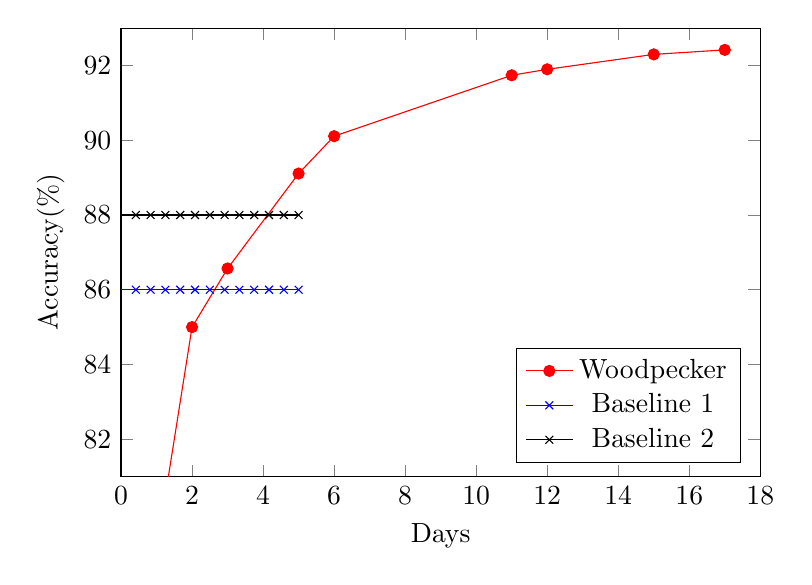
\begin{tikzpicture}
  \begin{axis}[
  		width=0.8\textwidth,
      	height=0.6\textwidth,
		xlabel={Days},
		ylabel= Accuracy(\%),
      	xmin= 0,
      	xmax= 18,
      	ymin=81,
      	ymax=93,
      	legend pos=south east],
	\addplot[color=red,mark=*] coordinates {
		(1,79)
		(2,85)
		(3,86.57)
		(5,89.11)
		(6,90.11)
		(11,91.74)
		(12,91.9)		
		(15,92.3)
		(17,92.42)
	};
	\addplot[color=blue,mark=x]{86};
	\addplot[mark=x]{88};

\legend{Woodpecker,Baseline 1, Baseline 2}
\end{axis}
\end{tikzpicture}
\caption{A plotting for Woodpecker's progress}
\label{ProcessPlot}
\end{center}
\end{figure}



\section{Methods}
In this section, we report the results of multiple methods we tried for feature extraction, dimension reduction, and classification. 

\subsection{Data preprocessing}

\subsection{Feature Selection}
To extract features from the raw word and image features, we experimented with multiple feature selection methods, including Information Gain, BNS
\subsection{Dimension Reduction}
\subsection{Classification}




\section{Discussion}
Working on this gender-classification project gave our team a chance reflected on what we have learned in class. Here is a short summary of things that have surprise us (or have taught us a lesson) 
\begin{itemize}
\item With different feature sets (especially they have various ranges and dimensions), feature selection and normalization have played an important role in improving the performances of our model. 
\item Last but not least, be careful with required formats..
\end{itemize} 

\section{Experiment Analysis}
In this section, we analyze the results of our experiments of multiple methods for feature extraction, dimension reduction, and classification. 
\subsection{Feature Selection/Extraction}

\subsection{Dimension Reduction}
\subsection{Classification}

\end{document}